\documentclass{article}
\usepackage{PreambleCommon}
\usepackage{minted}


\title{Assignment 4: Queues \\[5pt] Part 2: Shoppers \\[8pt] CS3305/W01 Data Structures}
\author{Casey Hampson}

\begin{document}
\maketitle


\section*{Program Output}
    The output is a little hard to parse (at least for me), so I'll describe the basic idea. What we see first is the initial five customers added to each line, then one more goes to 1, as it's the first available. Then someone checks out from line 3, making it the shortest line now, so the next customer goes to that line. Now 2-5 are the shortest, so it goes in order, and so on.
    \begin{center}
    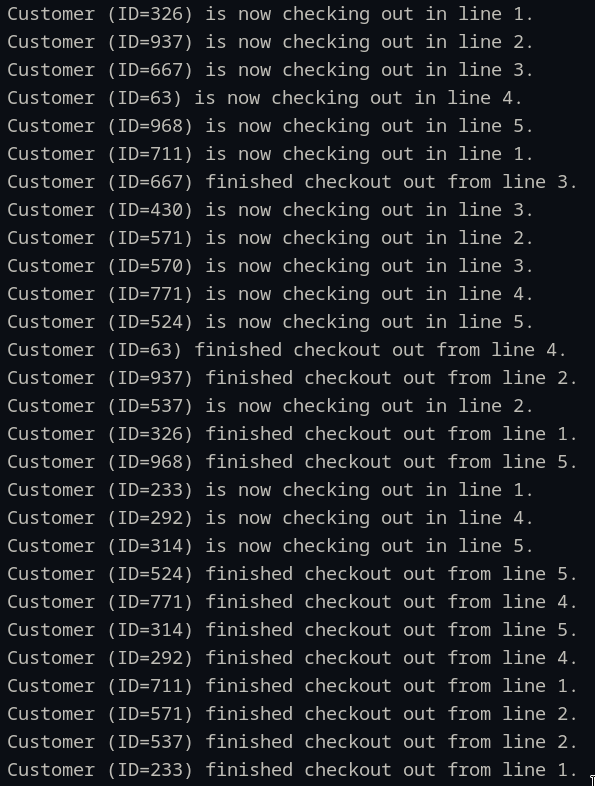
\includegraphics[width=0.5\textwidth]{./res/1.png}
    \end{center}





\pagebreak
\section*{Source Code}
\inputminted{java}{./P2.java}




\end{document}
